\chapter{ProvenByUsers}

\label{chap:ProvenByUsers}


ProvenByUsers is another online card sorting tool that allows users to quickly 
create studies and export the resulting data. Their user interface is 
minimalistic but adequate and their analysis tools are quite extensive.

\begin{figure}[tp] 
\centering
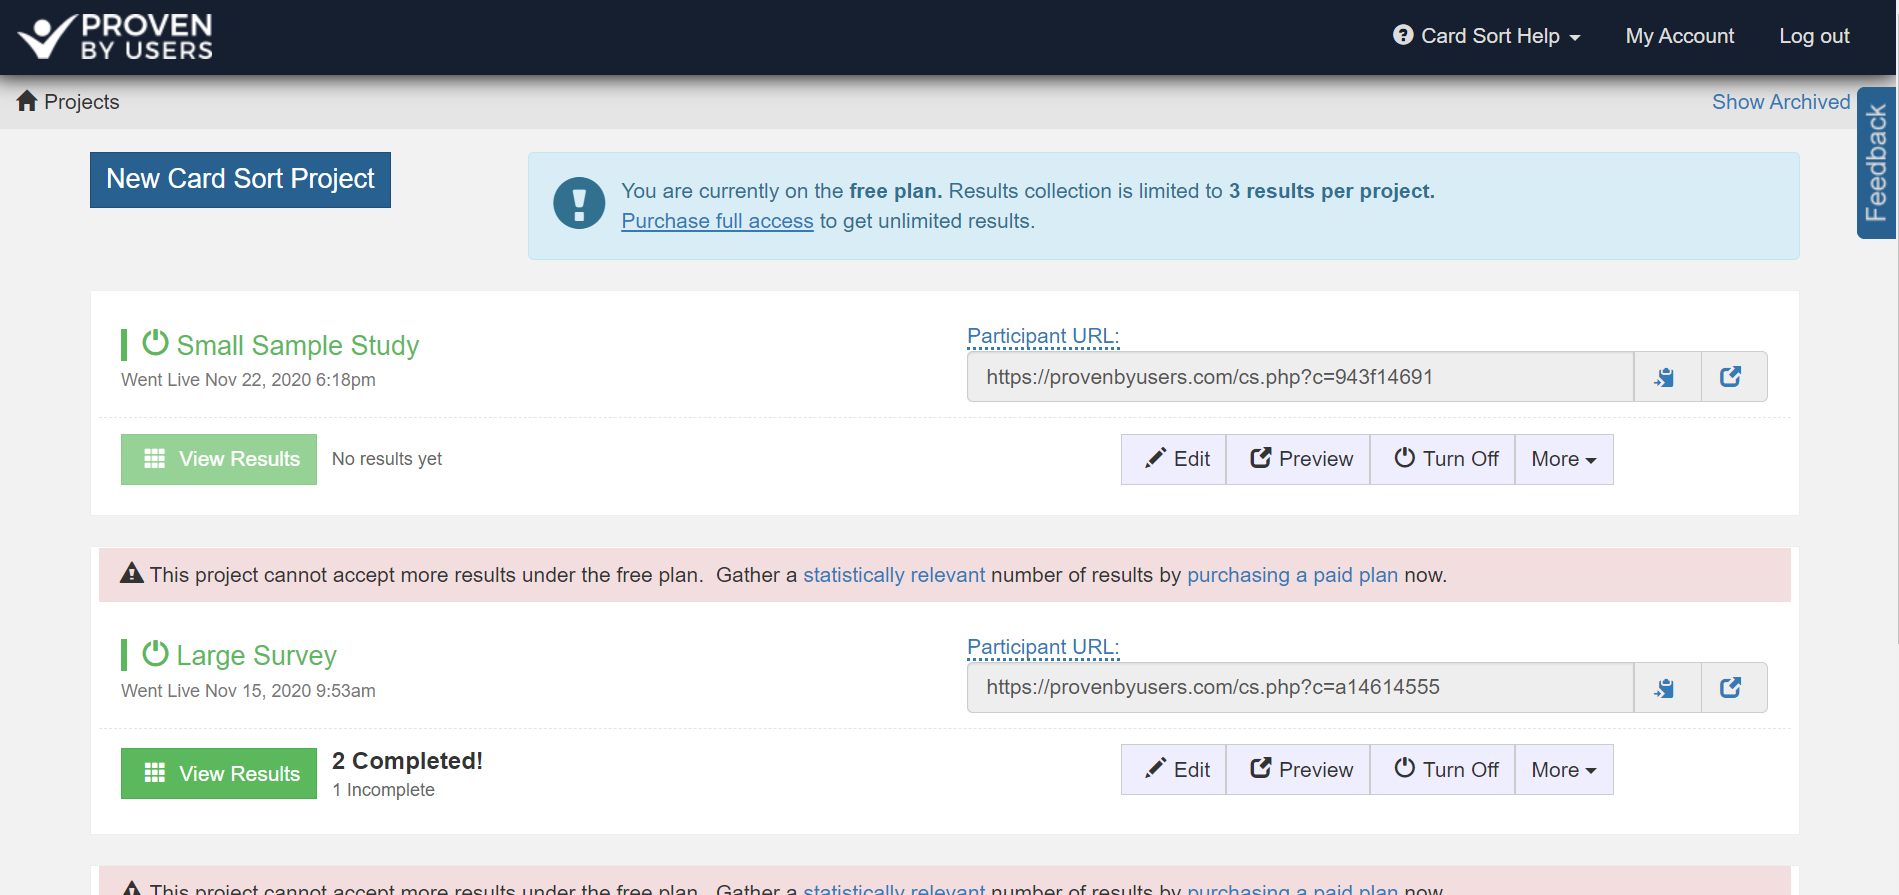
\includegraphics[keepaspectratio,width=\linewidth,height=\halfh]{images/provenbyusers-dashboard.png}
\caption[ProvenByUsers Application] { This is the base view in ProvenByUsers.
It shows an overview of your current and previous studies as well as the option
to create a new study.
\imgcredit{Screenshot was captured by Markus Ruplitsch using
\textcite{ProvenByUsers} on Google Chrome 84.} }
\label{fig:ProvenByUsers1}
\end{figure}


\section{Business Model}
All of their features can be accessed freely after creating an account, with the
only limitation being that only 3 results can be collected per survey. Since 3 
results are usually not enough, this means that a premium membership is necessary
for most purposes.

ProvenByUsers offers 3 different options for purchasing the option to have 
more than 3 participants per study. The first one costs \$39.95 for 30 days, 
the second one costs \$69.95 for 60 days and the last option costs \$399.95 
for one year. A screenshot of the dashboard can be found in figure 
~\ref{fig:ProvenByUsers1}.

\section{Card Sorting}
Creating a card sorting study is relatively simple when using ProvenByUsers.
 Users are presented with a number of different fields that can customize 
 options. They are sorted into different categories than can be accessed via a 
 menu bar to the left and can be filled out in any order. 

The only notable problem that was encountered during the creation of a study, was 
that it is not possible to import the cards or categories as files, but rather 
have to be copied and pasted into a text field. This is especially unintuitive 
if one wants to create a study with several layers of sub-categories as the 
text has to be in a specific format. 

However, that was the only problem and their documentation has a very detailed 
explanation of all the fields that have to be filled out. Overall, there are a 
lot of customization options, including questionaires before or after the 
survey, color and style choices and a number of messages that can be displayed 
at varying points before, during or after the survey. A screenshot of the card
sorting process can be found in figure ~\ref{fig:ProvenByUsers2}.

\begin{figure}[tp] 
\centering
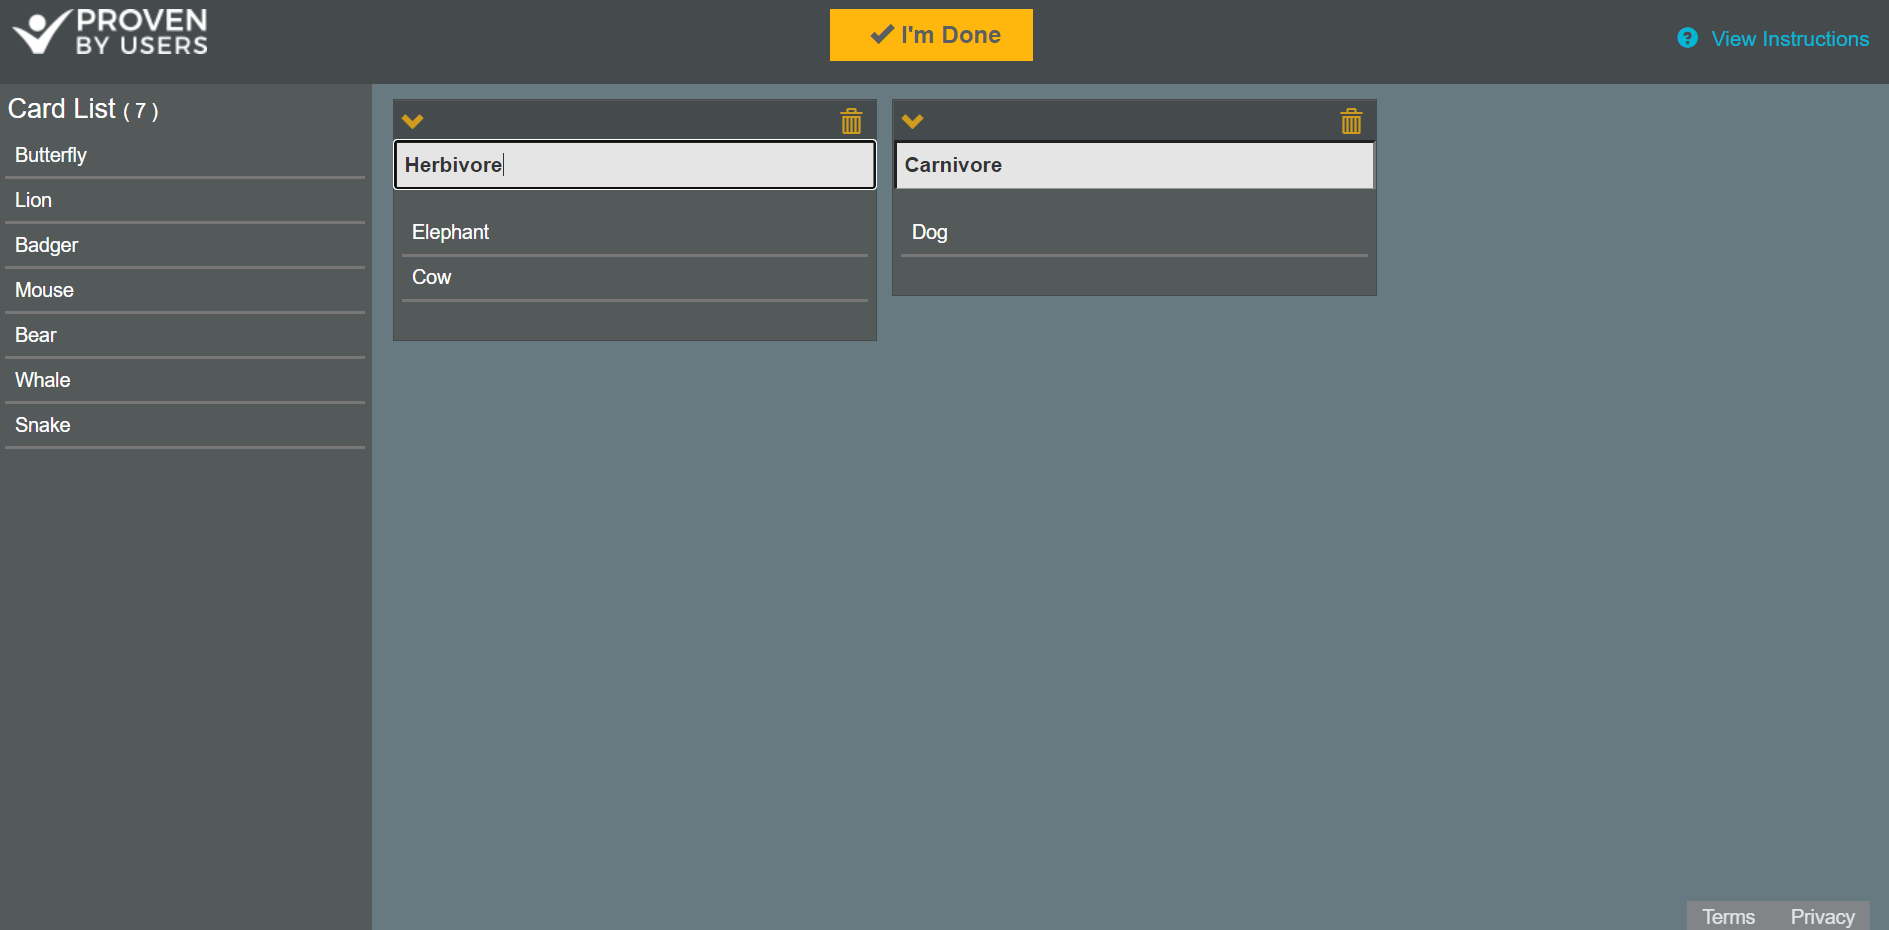
\includegraphics[keepaspectratio,width=\linewidth,height=\halfh]{images/provenbyusers-sorting.png}
\caption[ProvenByUsers Card Sorting] { This is a screenshot during the card
sorting process in ProvenByUsers.
\imgcredit{Screenshot was captured by Markus Ruplitsch using
\textcite{ProvenByUsers} on Google Chrome 84.} }
\label{fig:ProvenByUsers2}
\end{figure}


\section{Analytics}
Even before a study has closed, it is possible to review the results of every 
person who has participated in the study so far. ProvenByUsers allows users to 
view the data in a number of different ways.as well as some more analytical 
tools such as a similarity matrix, a dendrogram and a maximum agreement table. 
Users can be individually included or excluded in all of these results and all 
results, except the dendrogram, can be exported as either CSV or Syncaps
file format (see chapter \ref{chap:SynCaps}). A detailed summary of features 
can be viewed in table~\ref{tab:features-ProvenByUsers}

\begin{table}[tp]
\centering
\begin{tabularx}
{\linewidth}{|l|X|}
\hline \textbf{Feature/Characteristic} & \textbf{Availability in ProvenByUsers} \\ 
\hline Card Sorting & Open, closed and hybrid. \\ 
\hline Card Limit & None. \\
\hline Participant Limit & None. \\
\hline Analytics &  similarity matrix, dendrogram, maximum agreement table\\ 
\hline Documentation & Extremely detailed written documentation with a number 
of screenshots \\
\hline Business Model & Free or  \$ 39.95 for 30 days / \$ 69.95 for 60 days / 
\$ 399.95 for one year\\
\hline Import formats & None. All data needs to be entered by hand or copied as 
text.\\ 
\hline Export formats & .csv and SynCaps file format \\ 
\hline Sub-Categories & Yes. \\ 
\hline Playback of user-sessions & No. \\ 
\hline Data preparation & Allows inclusion / exclusion of specific users \\ 
\hline
\end{tabularx} 
\caption[Feature summary of ProvenByUsers] 
{ 
This table summarizes all the features and characteristics of ProvenByUsers
to provide an easy to read overview.
}
\label{tab:features-ProvenByUsers}
\end{table}

\section{Summary \& Ratings}
ProvenByUsers is relatively easy to use and offers a very detailed written 
documentation. There are numerous customization options when creating a 
study, as well as a good number of analysis tools. 

As with \textcite{UXtweak}, there are no major downsides to using this tool, but
because they only allow 3 participants per study, it is basically required to 
buy a premium membership. This time however, it is not possible to conduct 
smaller studies without paying, as 3 participants simply is not enough to make 
any statements with high confidence. The ratings can be found in table
~\ref{tab:rating-ProvenByUsers} and range from 0-5.


\begin{table}[tp] 
\centering 
\begin{tabularx}{\linewidth}{|X|X|X|X|X|}
\hline
Simplicity & Documentation & Features & Business Model & Average \\ 
\hline 
4 & 4 & 4 & 1 & 3.5 \\ 
\hline 
\end{tabularx} 
\caption[Ratings for ProvenByUsers] {
Ratings for ProvenByUsers including the average rating.
} 
\label{tab:rating-ProvenByUsers}
\end{table}



